\documentclass[11pt,oneside,a4paper,notitlepage]{article}

\usepackage[utf8]{inputenc}
\usepackage[ngerman]{babel}
\usepackage[margin=1.5cm]{geometry}

%kommentare, zitate, quellcode
\usepackage{verbatim}
%\fontfamily{sfdefault}
\renewcommand{\familydefault}{\sfdefault}
%
\usepackage{graphicx}
%fuer tabellen
\usepackage{tabularx}
\usepackage{tabulary}
%
%formatierung listen
\let\oldenumerate\enumerate
\renewcommand{\enumerate}{
  \oldenumerate
  \setlength{\itemsep}{1pt}
  \setlength{\parskip}{0pt}
  \setlength{\parsep}{0pt}
}

%
%referenzen und links
\usepackage{hyperref}
\hypersetup{
colorlinks=true,
linkcolor=cyan,
urlcolor=cyan,
hidelinks=false
}
%
% 
\renewcommand{\arraystretch}{1.5}
%

\begin{document}
%
\section{System \& Nutzerinformationen}

Zur Vorbereitung der Anforderungsanalyse werden hier einige Informationen zum System und deren Benutzer zusammengetragen.


\section{Systemprozess}
%
Ausgehend von \href{EISWS1516Howe_Domaenenrecherche.pdf}{Domänenrecherche (Prozess)} die Darstellung eines exemplarischen Verarbeitungsprozesses\\

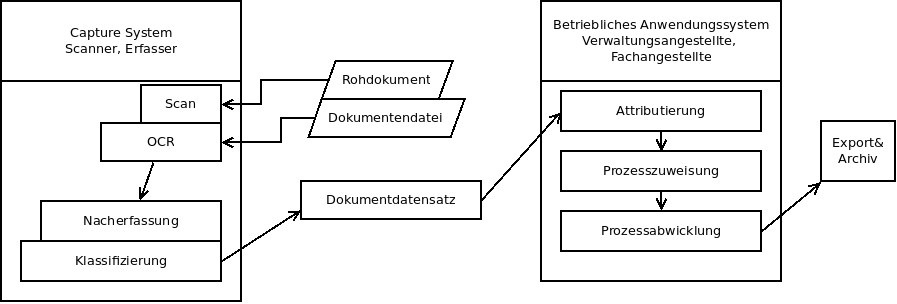
\includegraphics[width=\textwidth]{EISWS1516Howe_Prozess_deskriptiv.png}
\noindent
%
%
\section{Gesprächsprotokolle}


\subsection{Gespräch vom 22.10}
\subsubsection{Beteiligte Personen \& Abteilungen}
\label{subsec:gespraech_personen}

\paragraph*{Scanner}
Öffnen und Scannen analoge Eingangsdokumente, üblicherweise ungelernte Hilfskräfte, in kleineren Unternehmen zT auch die gleichen Personen die auch Erfassen, arbeiten an Scanstationen oder an einem Büroarbeitsplatz

\paragraph*{Erfasser}
%
Erfassen digitale Dokumente vollständig oder als Korrektur, der Nacherfassung, zu einer OCR Funktion. In kleineren Unternehmen: Buchhaltern oder Sekretären; mittelgroße Unternehmen: oft ungelernte Hilfkräfte, studentische Aushilfen; große Unternehmen: auslagern in dezidierte Erfassungszentren, ggf im Ausland. arbeiten an einem Büroarbeitsplatz, idR mit spezieller Erfassungsoftware

%
\paragraph*{Buchhalter}
Korrigieren ggf. erfasste Dokumente, übertragen in betriebliches Anwendungssystem: Buchhaltung, Dokumentenbearbeitungsfluss (Workflow), Archivsystem. Oft Steuerfachangestellte, Finanzbuchhalter oder eine Ausprägung der bürokaufmännischen Fachangestellten, seltener auch Studium oder Wirtschaftsprüfer, arbeiten an Büroarbeitsplatz, Schnittstelle zwischen Erfassung betrieblichem Prozess

%
\paragraph*{Fachabteilung}
je nach Unternehmensgröße und Struktur sehr vielfätig, unterschiedlich in den Dokumentenbearbeitungsfluss eingebunden, bearbeiten Ihren Teil des Geschäftsprozesses eines Dokuments. Oft fachbezogene Ausbildung oder Studium. Arbeiten idR. an Büroarbeitsplatz, haben abteilungs- projektbezogene Besprechungen. Übliche Fachabteilungen sind zb Marketing, IT, Personal, Logistik, Recht, Produktion, Montage, Finanzen.

%
\paragraph*{Abteilungsverantwortliche, Entscheider}
leitende Angestellte der Verwaltung, der Fachabteilungen sowie die Geschäftsführung. Überblicken und steuern ggf den Dokumentenarbeitsfluss, bewilligen Geschäftsvorgänge. Häufig fachbezogenes Studium oder auch Ausbildung und langjährige Berufserfahrung; Hintergrund Entscheider für Buchhaltung: zb Steuerfachangestellte, Controlling- oder Verwaltungs-Studium. Arbeiten an Büroarbeitsplatz, haben häufig Besprechungen im Rahmen der Fachabteilungen, Projekte oder Geschäftsführung.


\subsubsection{Dokumenttypen}
Im Allgemeinen viele mögliche Ausprägungen von Rechnungen, Lieferscheinen, Bestellungen oder Formularen, überwiegender Teil in allen Branchen sind Rechnungen.




%
\end{document}

